\PassOptionsToPackage{unicode=true}{hyperref} % options for packages loaded elsewhere
\PassOptionsToPackage{hyphens}{url}
%
\documentclass[11pt,]{article}
\usepackage{lmodern}
\usepackage{amssymb,amsmath}
\usepackage{ifxetex,ifluatex}
\usepackage{fixltx2e} % provides \textsubscript
\ifnum 0\ifxetex 1\fi\ifluatex 1\fi=0 % if pdftex
  \usepackage[T1]{fontenc}
  \usepackage[utf8]{inputenc}
  \usepackage{textcomp} % provides euro and other symbols
\else % if luatex or xelatex
  \usepackage{unicode-math}
  \defaultfontfeatures{Ligatures=TeX,Scale=MatchLowercase}
\fi
% use upquote if available, for straight quotes in verbatim environments
\IfFileExists{upquote.sty}{\usepackage{upquote}}{}
% use microtype if available
\IfFileExists{microtype.sty}{%
\usepackage[]{microtype}
\UseMicrotypeSet[protrusion]{basicmath} % disable protrusion for tt fonts
}{}
\IfFileExists{parskip.sty}{%
\usepackage{parskip}
}{% else
\setlength{\parindent}{0pt}
\setlength{\parskip}{6pt plus 2pt minus 1pt}
}
\usepackage{hyperref}
\hypersetup{
            pdftitle={VARS in R},
            pdfauthor={Arnald Puy},
            pdfborder={0 0 0},
            breaklinks=true}
\urlstyle{same}  % don't use monospace font for urls
\usepackage[margin=1in]{geometry}
\usepackage{color}
\usepackage{fancyvrb}
\newcommand{\VerbBar}{|}
\newcommand{\VERB}{\Verb[commandchars=\\\{\}]}
\DefineVerbatimEnvironment{Highlighting}{Verbatim}{commandchars=\\\{\}}
% Add ',fontsize=\small' for more characters per line
\usepackage{framed}
\definecolor{shadecolor}{RGB}{248,248,248}
\newenvironment{Shaded}{\begin{snugshade}}{\end{snugshade}}
\newcommand{\AlertTok}[1]{\textcolor[rgb]{0.94,0.16,0.16}{#1}}
\newcommand{\AnnotationTok}[1]{\textcolor[rgb]{0.56,0.35,0.01}{\textbf{\textit{#1}}}}
\newcommand{\AttributeTok}[1]{\textcolor[rgb]{0.77,0.63,0.00}{#1}}
\newcommand{\BaseNTok}[1]{\textcolor[rgb]{0.00,0.00,0.81}{#1}}
\newcommand{\BuiltInTok}[1]{#1}
\newcommand{\CharTok}[1]{\textcolor[rgb]{0.31,0.60,0.02}{#1}}
\newcommand{\CommentTok}[1]{\textcolor[rgb]{0.56,0.35,0.01}{\textit{#1}}}
\newcommand{\CommentVarTok}[1]{\textcolor[rgb]{0.56,0.35,0.01}{\textbf{\textit{#1}}}}
\newcommand{\ConstantTok}[1]{\textcolor[rgb]{0.00,0.00,0.00}{#1}}
\newcommand{\ControlFlowTok}[1]{\textcolor[rgb]{0.13,0.29,0.53}{\textbf{#1}}}
\newcommand{\DataTypeTok}[1]{\textcolor[rgb]{0.13,0.29,0.53}{#1}}
\newcommand{\DecValTok}[1]{\textcolor[rgb]{0.00,0.00,0.81}{#1}}
\newcommand{\DocumentationTok}[1]{\textcolor[rgb]{0.56,0.35,0.01}{\textbf{\textit{#1}}}}
\newcommand{\ErrorTok}[1]{\textcolor[rgb]{0.64,0.00,0.00}{\textbf{#1}}}
\newcommand{\ExtensionTok}[1]{#1}
\newcommand{\FloatTok}[1]{\textcolor[rgb]{0.00,0.00,0.81}{#1}}
\newcommand{\FunctionTok}[1]{\textcolor[rgb]{0.00,0.00,0.00}{#1}}
\newcommand{\ImportTok}[1]{#1}
\newcommand{\InformationTok}[1]{\textcolor[rgb]{0.56,0.35,0.01}{\textbf{\textit{#1}}}}
\newcommand{\KeywordTok}[1]{\textcolor[rgb]{0.13,0.29,0.53}{\textbf{#1}}}
\newcommand{\NormalTok}[1]{#1}
\newcommand{\OperatorTok}[1]{\textcolor[rgb]{0.81,0.36,0.00}{\textbf{#1}}}
\newcommand{\OtherTok}[1]{\textcolor[rgb]{0.56,0.35,0.01}{#1}}
\newcommand{\PreprocessorTok}[1]{\textcolor[rgb]{0.56,0.35,0.01}{\textit{#1}}}
\newcommand{\RegionMarkerTok}[1]{#1}
\newcommand{\SpecialCharTok}[1]{\textcolor[rgb]{0.00,0.00,0.00}{#1}}
\newcommand{\SpecialStringTok}[1]{\textcolor[rgb]{0.31,0.60,0.02}{#1}}
\newcommand{\StringTok}[1]{\textcolor[rgb]{0.31,0.60,0.02}{#1}}
\newcommand{\VariableTok}[1]{\textcolor[rgb]{0.00,0.00,0.00}{#1}}
\newcommand{\VerbatimStringTok}[1]{\textcolor[rgb]{0.31,0.60,0.02}{#1}}
\newcommand{\WarningTok}[1]{\textcolor[rgb]{0.56,0.35,0.01}{\textbf{\textit{#1}}}}
\usepackage{graphicx,grffile}
\makeatletter
\def\maxwidth{\ifdim\Gin@nat@width>\linewidth\linewidth\else\Gin@nat@width\fi}
\def\maxheight{\ifdim\Gin@nat@height>\textheight\textheight\else\Gin@nat@height\fi}
\makeatother
% Scale images if necessary, so that they will not overflow the page
% margins by default, and it is still possible to overwrite the defaults
% using explicit options in \includegraphics[width, height, ...]{}
\setkeys{Gin}{width=\maxwidth,height=\maxheight,keepaspectratio}
\setlength{\emergencystretch}{3em}  % prevent overfull lines
\providecommand{\tightlist}{%
  \setlength{\itemsep}{0pt}\setlength{\parskip}{0pt}}
\setcounter{secnumdepth}{5}
% Redefines (sub)paragraphs to behave more like sections
\ifx\paragraph\undefined\else
\let\oldparagraph\paragraph
\renewcommand{\paragraph}[1]{\oldparagraph{#1}\mbox{}}
\fi
\ifx\subparagraph\undefined\else
\let\oldsubparagraph\subparagraph
\renewcommand{\subparagraph}[1]{\oldsubparagraph{#1}\mbox{}}
\fi

% set default figure placement to htbp
\makeatletter
\def\fps@figure{htbp}
\makeatother

\usepackage[font=footnotesize]{caption}
\usepackage{dirtytalk}
\usepackage{booktabs}
\usepackage{tabulary}
\usepackage{enumitem}
\usepackage{lmodern}
\usepackage[T1]{fontenc}

\title{VARS in R}
\author{Arnald Puy}
\date{}

\begin{document}
\maketitle

\newpage

\begin{Shaded}
\begin{Highlighting}[]
\CommentTok{# PRELIMINARY FUNCTIONS -------------------------------------------------------}

\CommentTok{# Function to read in all required packages in one go:}
\NormalTok{loadPackages <-}\StringTok{ }\ControlFlowTok{function}\NormalTok{(x) \{}
  \ControlFlowTok{for}\NormalTok{(i }\ControlFlowTok{in}\NormalTok{ x) \{}
    \ControlFlowTok{if}\NormalTok{(}\OperatorTok{!}\KeywordTok{require}\NormalTok{(i, }\DataTypeTok{character.only =} \OtherTok{TRUE}\NormalTok{)) \{}
      \KeywordTok{install.packages}\NormalTok{(i, }\DataTypeTok{dependencies =} \OtherTok{TRUE}\NormalTok{)}
      \KeywordTok{library}\NormalTok{(i, }\DataTypeTok{character.only =} \OtherTok{TRUE}\NormalTok{)}
\NormalTok{    \}}
\NormalTok{  \}}
\NormalTok{\}}

\CommentTok{# Install development version of sensobol}
\NormalTok{remotes}\OperatorTok{::}\KeywordTok{install_github}\NormalTok{(}\StringTok{"arnaldpuy/sensobol"}\NormalTok{)}

\CommentTok{# Load the packages}
\KeywordTok{loadPackages}\NormalTok{(}\KeywordTok{c}\NormalTok{(}\StringTok{"tidyverse"}\NormalTok{, }\StringTok{"sensobol"}\NormalTok{, }\StringTok{"data.table"}\NormalTok{))}



\CommentTok{# Create custom theme}
\NormalTok{theme_AP <-}\StringTok{ }\ControlFlowTok{function}\NormalTok{() \{}
  \KeywordTok{theme_bw}\NormalTok{() }\OperatorTok{+}
\StringTok{    }\KeywordTok{theme}\NormalTok{(}\DataTypeTok{panel.grid.major =} \KeywordTok{element_blank}\NormalTok{(),}
          \DataTypeTok{panel.grid.minor =} \KeywordTok{element_blank}\NormalTok{(),}
          \DataTypeTok{legend.background =} \KeywordTok{element_rect}\NormalTok{(}\DataTypeTok{fill =} \StringTok{"transparent"}\NormalTok{,}
                                           \DataTypeTok{color =} \OtherTok{NA}\NormalTok{),}
          \DataTypeTok{legend.key =} \KeywordTok{element_rect}\NormalTok{(}\DataTypeTok{fill =} \StringTok{"transparent"}\NormalTok{,}
                                    \DataTypeTok{color =} \OtherTok{NA}\NormalTok{))}
\NormalTok{\}}

\CommentTok{# Set checkpoint}

\KeywordTok{dir.create}\NormalTok{(}\StringTok{".checkpoint"}\NormalTok{)}
\KeywordTok{library}\NormalTok{(}\StringTok{"checkpoint"}\NormalTok{)}

\KeywordTok{checkpoint}\NormalTok{(}\StringTok{"2020-03-09"}\NormalTok{, }
           \DataTypeTok{R.version =}\StringTok{"3.6.1"}\NormalTok{, }
           \DataTypeTok{checkpointLocation =} \KeywordTok{getwd}\NormalTok{())}
\end{Highlighting}
\end{Shaded}

\newpage

\begin{Shaded}
\begin{Highlighting}[]
\CommentTok{# FUNCTION TO CREATE STAR-VARS ------------------------------------------------}

\CommentTok{# CROSS-SECTIONS WITHOUT STAR CENTER-----------------------------}

\NormalTok{vars_matrices <-}\StringTok{ }\ControlFlowTok{function}\NormalTok{(N, params, h) \{}
\NormalTok{  out <-}\StringTok{ }\NormalTok{center <-}\StringTok{ }\NormalTok{sections <-}\StringTok{ }\NormalTok{A <-}\StringTok{ }\NormalTok{B <-}\StringTok{ }\NormalTok{AB <-}\StringTok{ }\NormalTok{X <-}\StringTok{ }\NormalTok{out <-}\StringTok{ }\KeywordTok{list}\NormalTok{()}
\NormalTok{  mat <-}\StringTok{ }\NormalTok{randtoolbox}\OperatorTok{::}\KeywordTok{sobol}\NormalTok{(}\DataTypeTok{n =}\NormalTok{ N, }\DataTypeTok{dim =} \KeywordTok{length}\NormalTok{(params))}
  \ControlFlowTok{for}\NormalTok{(i }\ControlFlowTok{in} \DecValTok{1}\OperatorTok{:}\KeywordTok{nrow}\NormalTok{(mat)) \{}
\NormalTok{    center[[i]] <-}\StringTok{ }\NormalTok{mat[i, ]}
\NormalTok{    sections[[i]] <-}\StringTok{ }\KeywordTok{sapply}\NormalTok{(center[[i]], }\ControlFlowTok{function}\NormalTok{(x) \{}
\NormalTok{      all <-}\StringTok{ }\KeywordTok{seq}\NormalTok{(x }\OperatorTok\StringTok{ }\NormalTok{h, }\DecValTok{1}\NormalTok{, h)}
\NormalTok{      non.zeros <-}\StringTok{ }\NormalTok{all[all}\OperatorTok{!=}\StringTok{ }\DecValTok{0}\NormalTok{] }\CommentTok{# Remove zeroes}
\NormalTok{    \})}
\NormalTok{    B[[i]] <-}\StringTok{ }\KeywordTok{sapply}\NormalTok{(}\DecValTok{1}\OperatorTok{:}\KeywordTok{ncol}\NormalTok{(mat), }\ControlFlowTok{function}\NormalTok{(x) }
\NormalTok{      sections[[i]][, x][}\OperatorTok{!}\NormalTok{sections[[i]][, x] }\OperatorTok\StringTok{ }\NormalTok{center[[i]][x]])}
\NormalTok{    A[[i]] <-}\StringTok{ }\KeywordTok{matrix}\NormalTok{(center[[i]], }\DataTypeTok{nrow =} \KeywordTok{nrow}\NormalTok{(B[[i]]), }
                     \DataTypeTok{ncol =} \KeywordTok{length}\NormalTok{(center[[i]]), }\DataTypeTok{byrow =} \OtherTok{TRUE}\NormalTok{)}
\NormalTok{    X[[i]] <-}\StringTok{ }\KeywordTok{rbind}\NormalTok{(A[[i]], B[[i]])}
    \ControlFlowTok{for}\NormalTok{(j }\ControlFlowTok{in} \DecValTok{1}\OperatorTok{:}\KeywordTok{ncol}\NormalTok{(A[[i]])) \{}
\NormalTok{      AB[[i]] <-}\StringTok{ }\NormalTok{A[[i]]}
\NormalTok{      AB[[i]][, j] <-}\StringTok{ }\NormalTok{B[[i]][, j]}
\NormalTok{      X[[i]] <-}\StringTok{ }\KeywordTok{rbind}\NormalTok{(X[[i]], AB[[i]])}
\NormalTok{    \}}
\NormalTok{    AB[[i]] <-}\StringTok{ }\NormalTok{X[[i]][(}\DecValTok{2} \OperatorTok{*}\StringTok{ }\KeywordTok{nrow}\NormalTok{(B[[i]]) }\OperatorTok{+}\StringTok{ }\DecValTok{1}\NormalTok{)}\OperatorTok{:}\KeywordTok{nrow}\NormalTok{(X[[i]]), ]}
\NormalTok{    out[[i]] <-}\StringTok{ }\KeywordTok{rbind}\NormalTok{(}\KeywordTok{unname}\NormalTok{(center[[i]]), AB[[i]])}
\NormalTok{  \}}
  \KeywordTok{return}\NormalTok{(}\KeywordTok{do.call}\NormalTok{(rbind, out))}
\NormalTok{\}}

\CommentTok{# Function to cut by size}
\NormalTok{CutBySize <-}\StringTok{ }\ControlFlowTok{function}\NormalTok{(m, block.size, }\DataTypeTok{nb =} \KeywordTok{ceiling}\NormalTok{(m }\OperatorTok{/}\StringTok{ }\NormalTok{block.size)) \{}
\NormalTok{  int <-}\StringTok{ }\NormalTok{m }\OperatorTok{/}\StringTok{ }\NormalTok{nb}
\NormalTok{  upper <-}\StringTok{ }\KeywordTok{round}\NormalTok{(}\DecValTok{1}\OperatorTok{:}\NormalTok{nb }\OperatorTok{*}\StringTok{ }\NormalTok{int)}
\NormalTok{  lower <-}\StringTok{ }\KeywordTok{c}\NormalTok{(}\DecValTok{1}\NormalTok{, upper[}\OperatorTok{-}\NormalTok{nb] }\OperatorTok{+}\StringTok{ }\DecValTok{1}\NormalTok{)}
\NormalTok{  size <-}\StringTok{ }\KeywordTok{c}\NormalTok{(upper[}\DecValTok{1}\NormalTok{], }\KeywordTok{diff}\NormalTok{(upper))}
  \KeywordTok{cbind}\NormalTok{(lower, upper, size)}
\NormalTok{\}}

\CommentTok{# Function to compute VARS-TI}
\NormalTok{vars_ti <-}\StringTok{ }\ControlFlowTok{function}\NormalTok{(Y, N, params, h) \{}
\NormalTok{  n.cross.points <-}\StringTok{ }\KeywordTok{length}\NormalTok{(params) }\OperatorTok{*}\StringTok{ }\NormalTok{((}\DecValTok{1} \OperatorTok{/}\StringTok{ }\NormalTok{h) }\OperatorTok{-}\StringTok{ }\DecValTok{1}\NormalTok{) }\OperatorTok{+}\StringTok{ }\DecValTok{1}
\NormalTok{  index.centers <-}\StringTok{ }\KeywordTok{seq}\NormalTok{(}\DecValTok{1}\NormalTok{, }\KeywordTok{length}\NormalTok{(Y), n.cross.points)}
\NormalTok{  mat <-}\StringTok{ }\KeywordTok{matrix}\NormalTok{(Y[}\OperatorTok{-}\NormalTok{index.centers], }\DataTypeTok{ncol =}\NormalTok{ N)}
\NormalTok{  indices <-}\StringTok{ }\KeywordTok{CutBySize}\NormalTok{(}\KeywordTok{nrow}\NormalTok{(mat), }\DataTypeTok{nb =} \KeywordTok{length}\NormalTok{(params))}
\NormalTok{  out <-}\StringTok{ }\KeywordTok{list}\NormalTok{()}
  \ControlFlowTok{for}\NormalTok{(i }\ControlFlowTok{in} \DecValTok{1}\OperatorTok{:}\KeywordTok{nrow}\NormalTok{(indices)) \{}
\NormalTok{    out[[i]] <-}\StringTok{ }\NormalTok{mat[indices[i, }\StringTok{"lower"}\NormalTok{]}\OperatorTok{:}\NormalTok{indices[i, }\StringTok{"upper"}\NormalTok{], ]}
\NormalTok{  \}}
\NormalTok{  d <-}\StringTok{ }\KeywordTok{lapply}\NormalTok{(}\DecValTok{1}\OperatorTok{:}\KeywordTok{length}\NormalTok{(params), }\ControlFlowTok{function}\NormalTok{(x) }
    \KeywordTok{lapply}\NormalTok{(}\DecValTok{1}\OperatorTok{:}\KeywordTok{ncol}\NormalTok{(out[[x]]), }\ControlFlowTok{function}\NormalTok{(j) \{}
\NormalTok{      da <-}\StringTok{ }\KeywordTok{c}\NormalTok{(out[[x]][, j][}\DecValTok{1}\NormalTok{], }
              \KeywordTok{rep}\NormalTok{(out[[x]][, j][}\OperatorTok{-}\KeywordTok{c}\NormalTok{(}\DecValTok{1}\NormalTok{, }\KeywordTok{length}\NormalTok{(out[[x]][, j]))], }\DataTypeTok{each =} \DecValTok{2}\NormalTok{), }
\NormalTok{              out[[x]][, j][}\KeywordTok{length}\NormalTok{(out[[x]][, j])])}
\NormalTok{    \}))}
\NormalTok{  out <-}\StringTok{ }\KeywordTok{lapply}\NormalTok{(d, }\ControlFlowTok{function}\NormalTok{(x) }\KeywordTok{lapply}\NormalTok{(x, }\ControlFlowTok{function}\NormalTok{(y) }\KeywordTok{matrix}\NormalTok{(y, }\DataTypeTok{nrow =} \KeywordTok{length}\NormalTok{(y) }\OperatorTok{/}\StringTok{ }\DecValTok{2}\NormalTok{, }\DataTypeTok{byrow =} \OtherTok{TRUE}\NormalTok{)))}
\NormalTok{  variogr <-}\StringTok{ }\KeywordTok{unlist}\NormalTok{(}\KeywordTok{lapply}\NormalTok{(out, }\ControlFlowTok{function}\NormalTok{(x) }\KeywordTok{lapply}\NormalTok{(x, }\ControlFlowTok{function}\NormalTok{(y) }
    \KeywordTok{mean}\NormalTok{(}\FloatTok{0.5} \OperatorTok{*}\StringTok{ }\NormalTok{(y[, }\DecValTok{1}\NormalTok{] }\OperatorTok{-}\StringTok{ }\NormalTok{y[, }\DecValTok{2}\NormalTok{]) }\OperatorTok{^}\StringTok{ }\DecValTok{2}\NormalTok{))) }\OperatorTok
\StringTok{      }\KeywordTok{lapply}\NormalTok{(., }\ControlFlowTok{function}\NormalTok{(x) }\KeywordTok{do.call}\NormalTok{(rbind, x)) }\OperatorTok
\StringTok{      }\KeywordTok{lapply}\NormalTok{(., mean))}
\NormalTok{  covariogr <-}\StringTok{ }\KeywordTok{unlist}\NormalTok{(}\KeywordTok{lapply}\NormalTok{(out, }\ControlFlowTok{function}\NormalTok{(x)}
    \KeywordTok{lapply}\NormalTok{(x, }\ControlFlowTok{function}\NormalTok{(y) }\KeywordTok{cov}\NormalTok{(y[, }\DecValTok{1}\NormalTok{], y[, }\DecValTok{2}\NormalTok{]))) }\OperatorTok
\StringTok{      }\KeywordTok{lapply}\NormalTok{(., }\ControlFlowTok{function}\NormalTok{(x) Rfast}\OperatorTok{::}\KeywordTok{colmeans}\NormalTok{(}\KeywordTok{do.call}\NormalTok{(rbind, x))))}
\NormalTok{  VY <-}\StringTok{ }\KeywordTok{var}\NormalTok{(Y[index.centers])}
\NormalTok{  Ti <-}\StringTok{ }\NormalTok{(variogr }\OperatorTok{+}\StringTok{ }\NormalTok{covariogr) }\OperatorTok{/}\StringTok{ }\NormalTok{VY}
\NormalTok{  output <-}\StringTok{ }\NormalTok{data.table}\OperatorTok{::}\KeywordTok{data.table}\NormalTok{(Ti)}
\NormalTok{  output[, }\StringTok{`}\DataTypeTok{:=}\StringTok{`}\NormalTok{(}\DataTypeTok{parameters =}\NormalTok{ params)]}
  \KeywordTok{return}\NormalTok{(output)}
\NormalTok{\}}


\CommentTok{# CROSS-SECTIONS WITH STAR CENTER ----------------------------------}

\NormalTok{vars_matrices_NEW <-}\StringTok{ }\ControlFlowTok{function}\NormalTok{(N, params, h) \{}
\NormalTok{  out <-}\StringTok{ }\NormalTok{center <-}\StringTok{ }\NormalTok{sections <-}\StringTok{ }\NormalTok{A <-}\StringTok{ }\NormalTok{B <-}\StringTok{ }\NormalTok{AB <-}\StringTok{ }\NormalTok{X <-}\StringTok{ }\NormalTok{out <-}\StringTok{ }\KeywordTok{list}\NormalTok{()}
\NormalTok{  mat <-}\StringTok{ }\NormalTok{randtoolbox}\OperatorTok{::}\KeywordTok{sobol}\NormalTok{(}\DataTypeTok{n =}\NormalTok{ N, }\DataTypeTok{dim =} \KeywordTok{length}\NormalTok{(params))}
  \ControlFlowTok{for}\NormalTok{(i }\ControlFlowTok{in} \DecValTok{1}\OperatorTok{:}\KeywordTok{nrow}\NormalTok{(mat)) \{}
\NormalTok{    center[[i]] <-}\StringTok{ }\NormalTok{mat[i, ]}
\NormalTok{    sections[[i]] <-}\StringTok{ }\KeywordTok{sapply}\NormalTok{(mat[i, ], }\ControlFlowTok{function}\NormalTok{(x) \{}
\NormalTok{      all <-}\StringTok{ }\KeywordTok{seq}\NormalTok{(x }\OperatorTok\StringTok{ }\NormalTok{h, }\DecValTok{1}\NormalTok{, h)}
\NormalTok{      non.zeros <-}\StringTok{ }\NormalTok{all[all}\OperatorTok{!=}\StringTok{ }\DecValTok{0}\NormalTok{] }\CommentTok{# Remove zeroes}
\NormalTok{    \})}
\NormalTok{    A[[i]] <-}\StringTok{ }\KeywordTok{matrix}\NormalTok{(mat[i, ], }\DataTypeTok{nrow =} \KeywordTok{nrow}\NormalTok{(sections[[i]]), }
                     \DataTypeTok{ncol =} \KeywordTok{ncol}\NormalTok{(mat), }\DataTypeTok{byrow =} \OtherTok{TRUE}\NormalTok{)}
\NormalTok{    X[[i]] <-}\StringTok{ }\KeywordTok{rbind}\NormalTok{(A[[i]], sections[[i]])}
    \ControlFlowTok{for}\NormalTok{(j }\ControlFlowTok{in} \DecValTok{1}\OperatorTok{:}\KeywordTok{ncol}\NormalTok{(A[[i]])) \{}
\NormalTok{      AB[[i]] <-}\StringTok{ }\NormalTok{A[[i]]}
\NormalTok{      AB[[i]][, j] <-}\StringTok{ }\NormalTok{sections[[i]][, j]}
\NormalTok{      X[[i]] <-}\StringTok{ }\KeywordTok{rbind}\NormalTok{(X[[i]], AB[[i]])}
\NormalTok{    \}}
\NormalTok{    AB[[i]] <-}\StringTok{ }\NormalTok{X[[i]][(}\DecValTok{2} \OperatorTok{*}\StringTok{ }\KeywordTok{nrow}\NormalTok{(sections[[i]]) }\OperatorTok{+}\StringTok{ }\DecValTok{1}\NormalTok{)}\OperatorTok{:}\KeywordTok{nrow}\NormalTok{(X[[i]]), ]}
\NormalTok{  \}}
\NormalTok{  star.vars <-}\StringTok{ }\KeywordTok{do.call}\NormalTok{(rbind, AB)}
\NormalTok{  tmp <-}\StringTok{ }\KeywordTok{lapply}\NormalTok{(}\DecValTok{1}\OperatorTok{:}\NormalTok{N, }\ControlFlowTok{function}\NormalTok{(x) }
    \KeywordTok{rowSums}\NormalTok{(star.vars }\OperatorTok{==}\StringTok{ }\NormalTok{mat[x, ][}\KeywordTok{col}\NormalTok{(star.vars)]) }\OperatorTok{==}\StringTok{ }\KeywordTok{ncol}\NormalTok{(star.vars)) }
\NormalTok{  indices.star.output <-}\StringTok{ }\KeywordTok{unlist}\NormalTok{(}\KeywordTok{lapply}\NormalTok{(}\DecValTok{1}\OperatorTok{:}\NormalTok{N, }\ControlFlowTok{function}\NormalTok{(x) }\KeywordTok{which}\NormalTok{(tmp[[x]] }\OperatorTok{==}\StringTok{ }\OtherTok{TRUE}\NormalTok{)[}\DecValTok{1}\NormalTok{]))}
  \KeywordTok{return}\NormalTok{(}\KeywordTok{list}\NormalTok{(star.vars, indices.star.output))}
\NormalTok{\}}

\NormalTok{pairs_tmp <-}\StringTok{ }\ControlFlowTok{function}\NormalTok{(x, h) \{}
\NormalTok{  da <-}\StringTok{ }\KeywordTok{list}\NormalTok{()}
  \ControlFlowTok{for}\NormalTok{(i }\ControlFlowTok{in} \DecValTok{1}\OperatorTok{:}\NormalTok{((}\DecValTok{1}\OperatorTok{/}\NormalTok{h) }\OperatorTok{-}\StringTok{ }\DecValTok{1}\NormalTok{)) \{}
\NormalTok{    da[[i]] <-}\StringTok{ }\KeywordTok{c}\NormalTok{(x[i], x[i}\OperatorTok{+}\DecValTok{1}\NormalTok{])}
\NormalTok{  \}}
\NormalTok{  out <-}\StringTok{ }\KeywordTok{do.call}\NormalTok{(rbind, da)}
  \KeywordTok{return}\NormalTok{(out)}
\NormalTok{\}}

\NormalTok{pairs_fun <-}\StringTok{ }\ControlFlowTok{function}\NormalTok{(x, h) \{}
\NormalTok{  da <-}\StringTok{ }\KeywordTok{list}\NormalTok{()}
  \ControlFlowTok{for}\NormalTok{(j }\ControlFlowTok{in} \DecValTok{1}\OperatorTok{:}\KeywordTok{ncol}\NormalTok{(x)) \{}
\NormalTok{    da[[j]] <-}\StringTok{ }\KeywordTok{pairs_tmp}\NormalTok{(x[, j], }\DataTypeTok{h =}\NormalTok{ h)}
\NormalTok{  \}}
  \KeywordTok{return}\NormalTok{(da)}
\NormalTok{\}}

\NormalTok{vars_ti_NEW <-}\StringTok{ }\ControlFlowTok{function}\NormalTok{(Y, N, indices.var, params, h) \{}
\NormalTok{  mat <-}\StringTok{ }\KeywordTok{matrix}\NormalTok{(Y, }\DataTypeTok{ncol =}\NormalTok{ N)}
\NormalTok{  indices <-}\StringTok{ }\KeywordTok{CutBySize}\NormalTok{(}\KeywordTok{nrow}\NormalTok{(mat), }\DataTypeTok{nb =} \KeywordTok{length}\NormalTok{(params))}
\NormalTok{  out <-}\StringTok{ }\KeywordTok{list}\NormalTok{()}
  \ControlFlowTok{for}\NormalTok{(i }\ControlFlowTok{in} \DecValTok{1}\OperatorTok{:}\KeywordTok{nrow}\NormalTok{(indices)) \{}
\NormalTok{    out[[i]] <-}\StringTok{ }\NormalTok{mat[indices[i, }\StringTok{"lower"}\NormalTok{]}\OperatorTok{:}\NormalTok{indices[i, }\StringTok{"upper"}\NormalTok{], ]}
\NormalTok{  \}}
\NormalTok{  d <-}\StringTok{ }\KeywordTok{lapply}\NormalTok{(out, }\ControlFlowTok{function}\NormalTok{(x) }\KeywordTok{pairs_fun}\NormalTok{(x, }\DataTypeTok{h =}\NormalTok{ h))}
\NormalTok{  variogr <-}\StringTok{ }\KeywordTok{unlist}\NormalTok{(}\KeywordTok{lapply}\NormalTok{(d, }\ControlFlowTok{function}\NormalTok{(x) }\KeywordTok{lapply}\NormalTok{(x, }\ControlFlowTok{function}\NormalTok{(y) }
    \KeywordTok{mean}\NormalTok{(}\FloatTok{0.5} \OperatorTok{*}\StringTok{ }\NormalTok{(y[, }\DecValTok{1}\NormalTok{] }\OperatorTok{-}\StringTok{ }\NormalTok{y[, }\DecValTok{2}\NormalTok{]) }\OperatorTok{^}\StringTok{ }\DecValTok{2}\NormalTok{))) }\OperatorTok
\StringTok{      }\KeywordTok{lapply}\NormalTok{(., }\ControlFlowTok{function}\NormalTok{(x) }\KeywordTok{do.call}\NormalTok{(rbind, x)) }\OperatorTok
\StringTok{      }\KeywordTok{lapply}\NormalTok{(., mean))}
\NormalTok{  covariogr <-}\StringTok{ }\KeywordTok{unlist}\NormalTok{(}\KeywordTok{lapply}\NormalTok{(d, }\ControlFlowTok{function}\NormalTok{(x)}
    \KeywordTok{lapply}\NormalTok{(x, }\ControlFlowTok{function}\NormalTok{(y) }\KeywordTok{cov}\NormalTok{(y[, }\DecValTok{1}\NormalTok{], y[, }\DecValTok{2}\NormalTok{]))) }\OperatorTok
\StringTok{      }\KeywordTok{lapply}\NormalTok{(., }\ControlFlowTok{function}\NormalTok{(x) Rfast}\OperatorTok{::}\KeywordTok{colmeans}\NormalTok{(}\KeywordTok{do.call}\NormalTok{(rbind, x))))}
\NormalTok{  VY <-}\StringTok{ }\KeywordTok{var}\NormalTok{(Y[indices.var])}
\NormalTok{  Ti <-}\StringTok{ }\NormalTok{(variogr }\OperatorTok{+}\StringTok{ }\NormalTok{covariogr) }\OperatorTok{/}\StringTok{ }\NormalTok{VY}
\NormalTok{  output <-}\StringTok{ }\NormalTok{data.table}\OperatorTok{::}\KeywordTok{data.table}\NormalTok{(Ti)}
\NormalTok{  output[, }\StringTok{`}\DataTypeTok{:=}\StringTok{`}\NormalTok{(}\DataTypeTok{parameters =}\NormalTok{ params)]}
  \KeywordTok{return}\NormalTok{(output)}
\NormalTok{\}}
\end{Highlighting}
\end{Shaded}

\begin{Shaded}
\begin{Highlighting}[]
\CommentTok{# COMPARE RESULTS  ------------------------------------------------------------}

\NormalTok{vars_type <-}\StringTok{ }\KeywordTok{c}\NormalTok{(}\StringTok{"With"}\NormalTok{, }\StringTok{"Without"}\NormalTok{)}
\NormalTok{test_functions <-}\StringTok{ }\KeywordTok{c}\NormalTok{(}\StringTok{"Ishigami"}\NormalTok{, }\StringTok{"Sobol' G"}\NormalTok{, }\StringTok{"Morris"}\NormalTok{)}
\NormalTok{N <-}\StringTok{ }\DecValTok{200}
\NormalTok{h <-}\StringTok{ }\FloatTok{0.2}

\CommentTok{# Run model}
\NormalTok{mat <-}\StringTok{ }\NormalTok{Y <-}\StringTok{ }\NormalTok{ind <-}\StringTok{ }\KeywordTok{list}\NormalTok{()}
\ControlFlowTok{for}\NormalTok{(i }\ControlFlowTok{in}\NormalTok{ test_functions) \{}
  \ControlFlowTok{for}\NormalTok{(j }\ControlFlowTok{in}\NormalTok{ vars_type) \{}
    \ControlFlowTok{if}\NormalTok{(i }\OperatorTok{==}\StringTok{ "Ishigami"}\NormalTok{) \{}
\NormalTok{      k <-}\StringTok{ }\DecValTok{3}
\NormalTok{      modelRun <-}\StringTok{ }\NormalTok{sensobol}\OperatorTok{::}\NormalTok{ishigami_Fun}
\NormalTok{    \} }\ControlFlowTok{else} \ControlFlowTok{if}\NormalTok{(i }\OperatorTok{==}\StringTok{ "Sobol' G"}\NormalTok{) \{}
\NormalTok{      k <-}\StringTok{ }\DecValTok{8}
\NormalTok{      modelRun <-}\StringTok{ }\NormalTok{sensobol}\OperatorTok{::}\NormalTok{sobol_Fun}
\NormalTok{    \} }\ControlFlowTok{else} \ControlFlowTok{if}\NormalTok{(i }\OperatorTok{==}\StringTok{ "Morris"}\NormalTok{) \{}
\NormalTok{      k <-}\StringTok{ }\DecValTok{20}
\NormalTok{      modelRun <-}\StringTok{ }\NormalTok{sensitivity}\OperatorTok{::}\NormalTok{morris.fun}
\NormalTok{    \}}
    \ControlFlowTok{if}\NormalTok{(j }\OperatorTok{==}\StringTok{ "With"}\NormalTok{) \{}
\NormalTok{      mat[[i]][[j]] <-}\StringTok{ }\KeywordTok{vars_matrices_NEW}\NormalTok{(}\DataTypeTok{N =}\NormalTok{ N, }
                                         \DataTypeTok{params =} \KeywordTok{paste}\NormalTok{(}\StringTok{"X"}\NormalTok{, }\DecValTok{1}\OperatorTok{:}\NormalTok{k, }\DataTypeTok{sep =} \StringTok{""}\NormalTok{), }
                                         \DataTypeTok{h =}\NormalTok{ h)}
\NormalTok{      Y[[i]][[j]] <-}\StringTok{ }\KeywordTok{modelRun}\NormalTok{(mat[[i]][[j]][[}\DecValTok{1}\NormalTok{]])}
\NormalTok{      ind[[i]][[j]] <-}\StringTok{ }\KeywordTok{vars_ti_NEW}\NormalTok{(}\DataTypeTok{Y =}\NormalTok{ Y[[i]][[j]], }
                                   \DataTypeTok{N =}\NormalTok{ N, }
                                   \DataTypeTok{indices.var =}\NormalTok{ mat[[i]][[j]][[}\DecValTok{2}\NormalTok{]], }
                                   \DataTypeTok{params =} \KeywordTok{paste}\NormalTok{(}\StringTok{"X"}\NormalTok{, }\DecValTok{1}\OperatorTok{:}\NormalTok{k, }\DataTypeTok{sep =} \StringTok{""}\NormalTok{), }
                                   \DataTypeTok{h =}\NormalTok{ h)}
\NormalTok{    \} }\ControlFlowTok{else} \ControlFlowTok{if}\NormalTok{(j }\OperatorTok{==}\StringTok{ "Without"}\NormalTok{) \{}
\NormalTok{      mat[[i]][[j]] <-}\StringTok{ }\KeywordTok{vars_matrices}\NormalTok{(}\DataTypeTok{N =}\NormalTok{ N, }
                                     \DataTypeTok{params =} \KeywordTok{paste}\NormalTok{(}\StringTok{"X"}\NormalTok{, }\DecValTok{1}\OperatorTok{:}\NormalTok{k, }\DataTypeTok{sep =} \StringTok{""}\NormalTok{), }
                                     \DataTypeTok{h =}\NormalTok{ h)}
\NormalTok{      Y[[i]][[j]] <-}\StringTok{ }\KeywordTok{modelRun}\NormalTok{(mat[[i]][[j]])}
\NormalTok{      ind[[i]][[j]] <-}\StringTok{ }\KeywordTok{vars_ti}\NormalTok{(}\DataTypeTok{Y =}\NormalTok{ Y[[i]][[j]], }
                                   \DataTypeTok{N =}\NormalTok{ N, }
                                   \DataTypeTok{params =} \KeywordTok{paste}\NormalTok{(}\StringTok{"X"}\NormalTok{, }\DecValTok{1}\OperatorTok{:}\NormalTok{k, }\DataTypeTok{sep =} \StringTok{""}\NormalTok{), }
                                   \DataTypeTok{h =}\NormalTok{ h)}
\NormalTok{    \}}
\NormalTok{  \}}
\NormalTok{\}}
\end{Highlighting}
\end{Shaded}

\begin{verbatim}
## Registered S3 method overwritten by 'sensitivity':
##   method    from 
##   print.src dplyr
\end{verbatim}

\begin{Shaded}
\begin{Highlighting}[]
\CommentTok{# PLOT RESULTS ----------------------------------------------------------------}

\KeywordTok{lapply}\NormalTok{(ind, }\ControlFlowTok{function}\NormalTok{(x) }\KeywordTok{rbindlist}\NormalTok{(x, }\DataTypeTok{idcol =} \StringTok{"Type"}\NormalTok{)) }\OperatorTok
\StringTok{  }\KeywordTok{rbindlist}\NormalTok{(., }\DataTypeTok{idcol =} \StringTok{"Function"}\NormalTok{) }\OperatorTok
\StringTok{  }\NormalTok{.[, parameters}\OperatorTok{:}\ErrorTok{=}\StringTok{ }\KeywordTok{factor}\NormalTok{(parameters, }\DataTypeTok{levels =} \KeywordTok{paste}\NormalTok{(}\StringTok{"X"}\NormalTok{, }\DecValTok{1}\OperatorTok{:}\DecValTok{20}\NormalTok{, }\DataTypeTok{sep =} \StringTok{""}\NormalTok{))] }\OperatorTok
\StringTok{  }\NormalTok{.[, Function}\OperatorTok{:}\ErrorTok{=}\StringTok{ }\KeywordTok{factor}\NormalTok{(Function, }\DataTypeTok{levels =}\NormalTok{ test_functions)] }\OperatorTok
\StringTok{  }\KeywordTok{ggplot}\NormalTok{(., }\KeywordTok{aes}\NormalTok{(parameters, Ti, }\DataTypeTok{fill =}\NormalTok{ Type)) }\OperatorTok{+}
\StringTok{  }\KeywordTok{geom_bar}\NormalTok{(}\DataTypeTok{stat =} \StringTok{"identity"}\NormalTok{,}
           \DataTypeTok{position =} \KeywordTok{position_dodge}\NormalTok{(}\FloatTok{0.7}\NormalTok{),}
           \DataTypeTok{color =} \StringTok{"black"}\NormalTok{) }\OperatorTok{+}
\StringTok{  }\KeywordTok{scale_fill_discrete}\NormalTok{(}\DataTypeTok{name =} \KeywordTok{expression}\NormalTok{(}\KeywordTok{paste}\NormalTok{(}\StringTok{"VARS "}\OperatorTok{~}\NormalTok{T[}\KeywordTok{italic}\NormalTok{(i)])),}
                      \DataTypeTok{labels =} \KeywordTok{c}\NormalTok{(}\StringTok{"With star center"}\NormalTok{, }\StringTok{"Without star center"}\NormalTok{)) }\OperatorTok{+}
\StringTok{  }\KeywordTok{facet_grid}\NormalTok{(}\OperatorTok{~}\NormalTok{Function,}
             \DataTypeTok{scales =} \StringTok{"free_x"}\NormalTok{,}
             \DataTypeTok{space =} \StringTok{"free_x"}\NormalTok{) }\OperatorTok{+}
\StringTok{  }\KeywordTok{labs}\NormalTok{(}\DataTypeTok{x =} \StringTok{""}\NormalTok{,}
       \DataTypeTok{y =} \KeywordTok{expression}\NormalTok{(T[}\KeywordTok{italic}\NormalTok{(i)])) }\OperatorTok{+}
\StringTok{  }\KeywordTok{theme_AP}\NormalTok{() }\OperatorTok{+}
\StringTok{  }\KeywordTok{theme}\NormalTok{(}\DataTypeTok{axis.text.x =} \KeywordTok{element_text}\NormalTok{(}\DataTypeTok{size =} \FloatTok{6.5}\NormalTok{),}
        \DataTypeTok{legend.position =} \StringTok{"top"}\NormalTok{) }\OperatorTok{+}
\StringTok{  }\KeywordTok{guides}\NormalTok{(}\DataTypeTok{fill =} \KeywordTok{guide_legend}\NormalTok{(}\DataTypeTok{nrow =} \DecValTok{3}\NormalTok{,}
                             \DataTypeTok{byrow =} \OtherTok{TRUE}\NormalTok{))}
\end{Highlighting}
\end{Shaded}

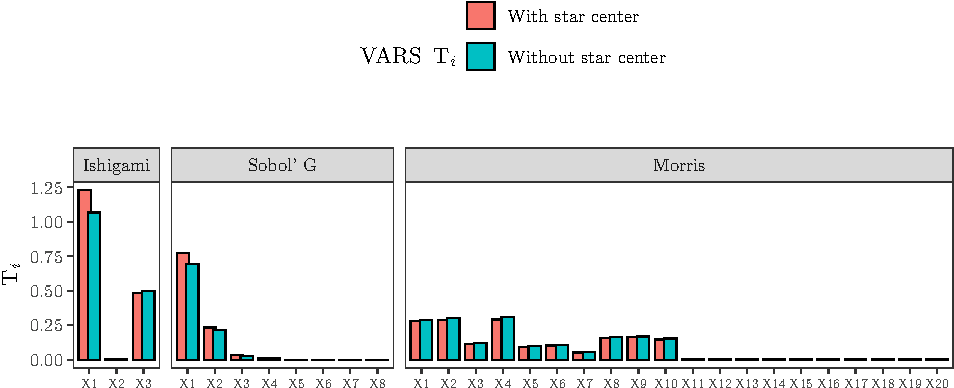
\includegraphics{code_vars_design_files/figure-latex/plot-1.pdf}

\end{document}
